
\appendix

\section{Appendix}
\label{sec:appendix}

\subsection{Fine-tuning Configuration for LLM Judges}
\label{sec:finetuning_configuration}

For our loss function used in LLM judge training, we selected cross-entropy loss using Adam \cite{kingma2017adam}. 
For our classification head, we use a single linear classification layer and apply a 0.1 dropout to the input, which is the final hidden state of the [CLS] token.
For our learning schedule, we use linear warmup and linear decay \cite{howard-ruder-2018-universal} with a 5e-6 learning rate and a 32 training batch size across all experimental configurations.

\subsection{GPT Prompting for Context Relevance Scoring}
\label{sec:gpt_prompting_for_context_relevance_scoring}

For the NQ, HotpotQA, MultiRC, and ReCoRD datasets, we use 8 few-shot examples with the following prompt to score context relevance:

\begin{itemize}
    \item Given the following question and document, you must analyze the provided document and determine whether it is sufficient for answering the question. 
    In your evaluation, you should consider the content of the document and how it relates to the provided question. 
    Output your final verdict by strictly following this format: "[[Yes]]" if the document is sufficient and "[[No]]" if the document provided is not sufficient. 
    Do not provide any additional explanation for your decision.
    
    Question: <\textit{few-shot example here}>
    
    Document: <\textit{few-shot example here}>
    
\end{itemize}

For FEVER, we use the following prompt to score context relevance:

\begin{itemize}
    \item You are an expert fact-checking agent. Given the following statement and document, you must analyze the provided document and determine whether it is sufficient for determining the statement's factuality. In your evaluation, you should consider the content of the document and how it relates to the provided statement's factuality. Output your final verdict by strictly following this format: "[[Yes]]" if the document is sufficient and "[[No]]" if the document is not sufficient. Do not provide any additional explanation for your decision.
    
    Statement: <\textit{few-shot example here}>
    
    Document: <\textit{few-shot example here}>
    
\end{itemize}

For WoW, we use the following prompt to score context relevance:

\begin{itemize}
    \item You are an expert dialogue agent. Given the following dialogue and document, you must analyze the provided document and determine whether it is relevant for responding to the dialogue. In your evaluation, you should consider the content of the document and how it relates to the provided dialogue. Output your final verdict by strictly following this format: "[[Yes]]" if the document is relevant and "[[No]]" if the document provided is not relevant. Do not provide any additional explanation for your decision.

    Dialogue: <\textit{few-shot example here}>
    
    Document: <\textit{few-shot example here}>
    
\end{itemize}



\subsection{GPT Prompting for Answer Faithfulness Scoring}
\label{sec:gpt_prompting_for_answer_faithfulness_scoring}

For the NQ, HotpotQA, MultiRC, and ReCoRD datasets, we use 8 few-shot examples with the following prompt to score answer faithfulness:

\begin{itemize}
    \item Given the following question, document, and answer, you must analyze the provided answer and determine whether it is faithful to the contents of the document. The answer must not offer new information beyond the context provided in the document. The answer also must not contradict information provided in the document. Output your final verdict by strictly following this format: "[[Yes]]" if the answer is faithful to the document and "[[No]]" if the answer is not faithful to the document. Do not provide any additional explanation for your decision.

    Question: <\textit{few-shot example here}>
    
    Document: <\textit{few-shot example here}>

    Answer: <\textit{few-shot example here}>

    
\end{itemize}

For FEVER, we change the word "question" in the prompt to "statement". 
For WoW, we change the word "question" in the prompt to "dialogue".

\subsection{GPT Prompting for Answer Relevance Scoring}
\label{sec:gpt_prompting_for_answer_relevance_scoring}

For the NQ, HotpotQA, MultiRC, and ReCoRD datasets, we use 8 few-shot examples with the following prompt to score answer relevance:

\begin{itemize}
    \item Given the following question, document, and answer, you must analyze the provided answer and document before determining whether the answer is relevant for the provided question. In your evaluation, you should consider whether the answer addresses all aspects of the question and provides only correct information from the document for answering the question. Output your final verdict by strictly following this format: "[[Yes]]" if the answer is relevant for the given question and "[[No]]" if the answer is not relevant for the given question. Do not provide any additional explanation for your decision.

    Question: <\textit{few-shot example here}>
    
    Document: <\textit{few-shot example here}>

    Answer: <\textit{few-shot example here}>
\end{itemize}

For FEVER, we change the word "question" in the prompt to "statement". 
For WoW, we change the word "question" in the prompt to "dialogue".

\subsection{Prompting for Generation of Synthetic Queries and Answers}
\label{sec:flan_generate_synth_data}

To generate synthetic queries and answers using FLAN-T5, we use the following prompt and provide 5 few-shot examples:

\begin{itemize}
    \item Example N

    Question: <\textit{few-shot example here}>

    Document: <\textit{few-shot example here}>

    Answer: <\textit{few-shot example here}>
    
\end{itemize}

We use the same prompting structure for generating incorrect or contradictory answers; we simply swap out the few-shot examples to be incorrect or contradictory instead.

\subsection{Synthetic Query and Answer Generation}
\label{sec:generate_synthetic_data}

For generating our synthetic questions, we use the following prompt for FLAN-T5 XXL:

\begin{itemize}
    \item Example \#1
    
    Document: <\textit{few-shot example here}>
    
    Query: <\textit{few-shot example here}>
    
    Example \#2
    
    Document: <\textit{few-shot example here}>
    
    Query: <\textit{few-shot example here}>

    Example \#3
    
    Document: <\textit{few-shot example here}>
    
    Query: <\textit{few-shot example here}>

    Example \#4
    
    Document: <\textit{in-domain passage}>
    
    Query: 
\end{itemize}

For generating our synthetic answers, we use the following prompt for FLAN-T5 XXL:

\begin{itemize}
    \item Example \#1

    Query: <\textit{few-shot example here}>
    
    Document: <\textit{few-shot example here}>
    
    Answer: <\textit{few-shot example here}>
    
    Example \#2
    
    Query: <\textit{few-shot example here}>
    
    Document: <\textit{few-shot example here}>
    
    Answer: <\textit{few-shot example here}>

    Example \#3
    
    Query: <\textit{few-shot example here}>
    
    Document: <\textit{few-shot example here}>
    
    Answer: <\textit{few-shot example here}>

    Example \#4
    
    Query: <\textit{synthetic query here}>
    
    Document: <\textit{in-domain passage here}>
    
    Answer:
\end{itemize}



\begin{figure*}[tp!]
   \centering
   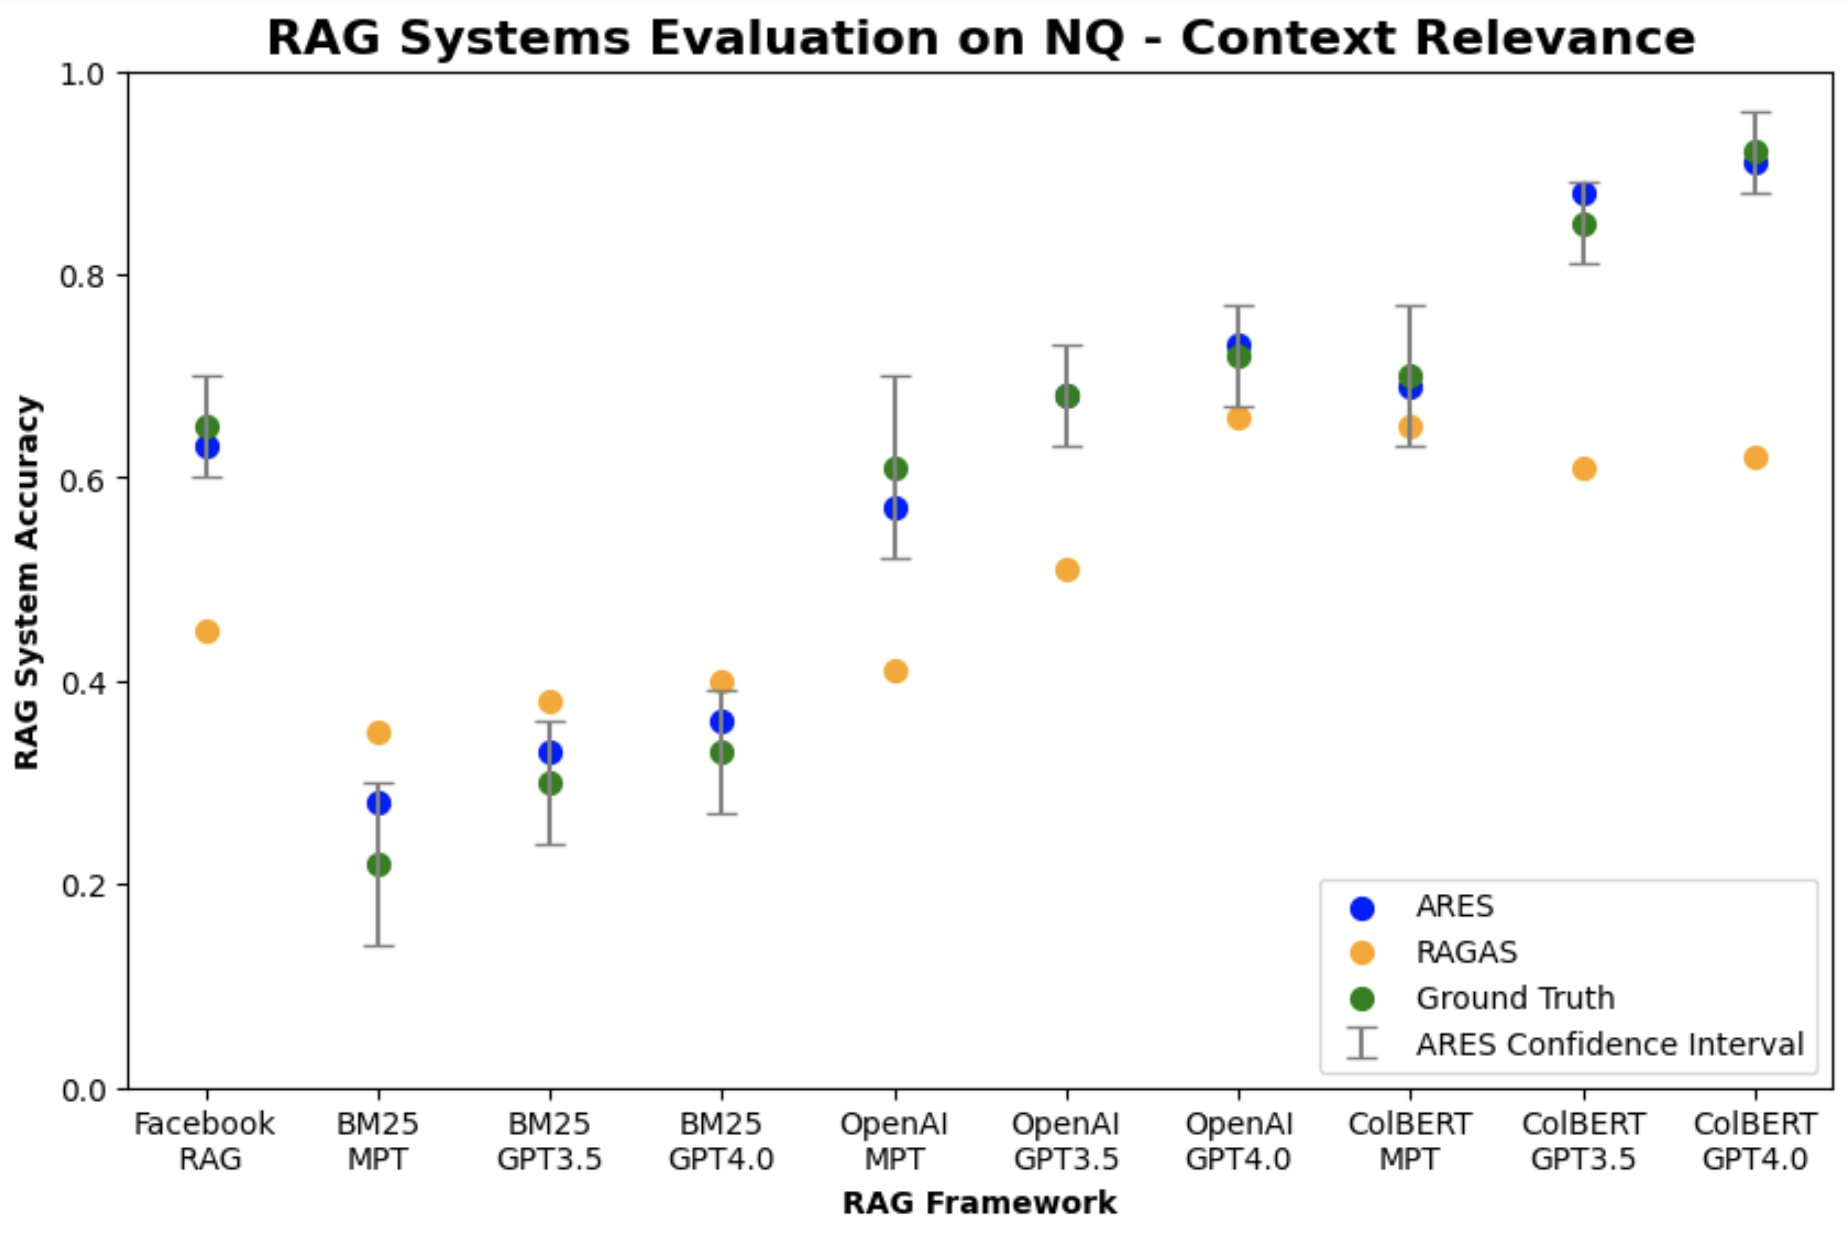
\includegraphics[width=0.8\linewidth]{Tables/NQ_ContextRelevance.png}
   \caption{\textbf{RAG Systems Evaluation on NQ - Context Relevance}}
   \label{fig:nq_context_relevance_real_rag}
\end{figure*}





\begin{figure*}[tp!]
   \centering
   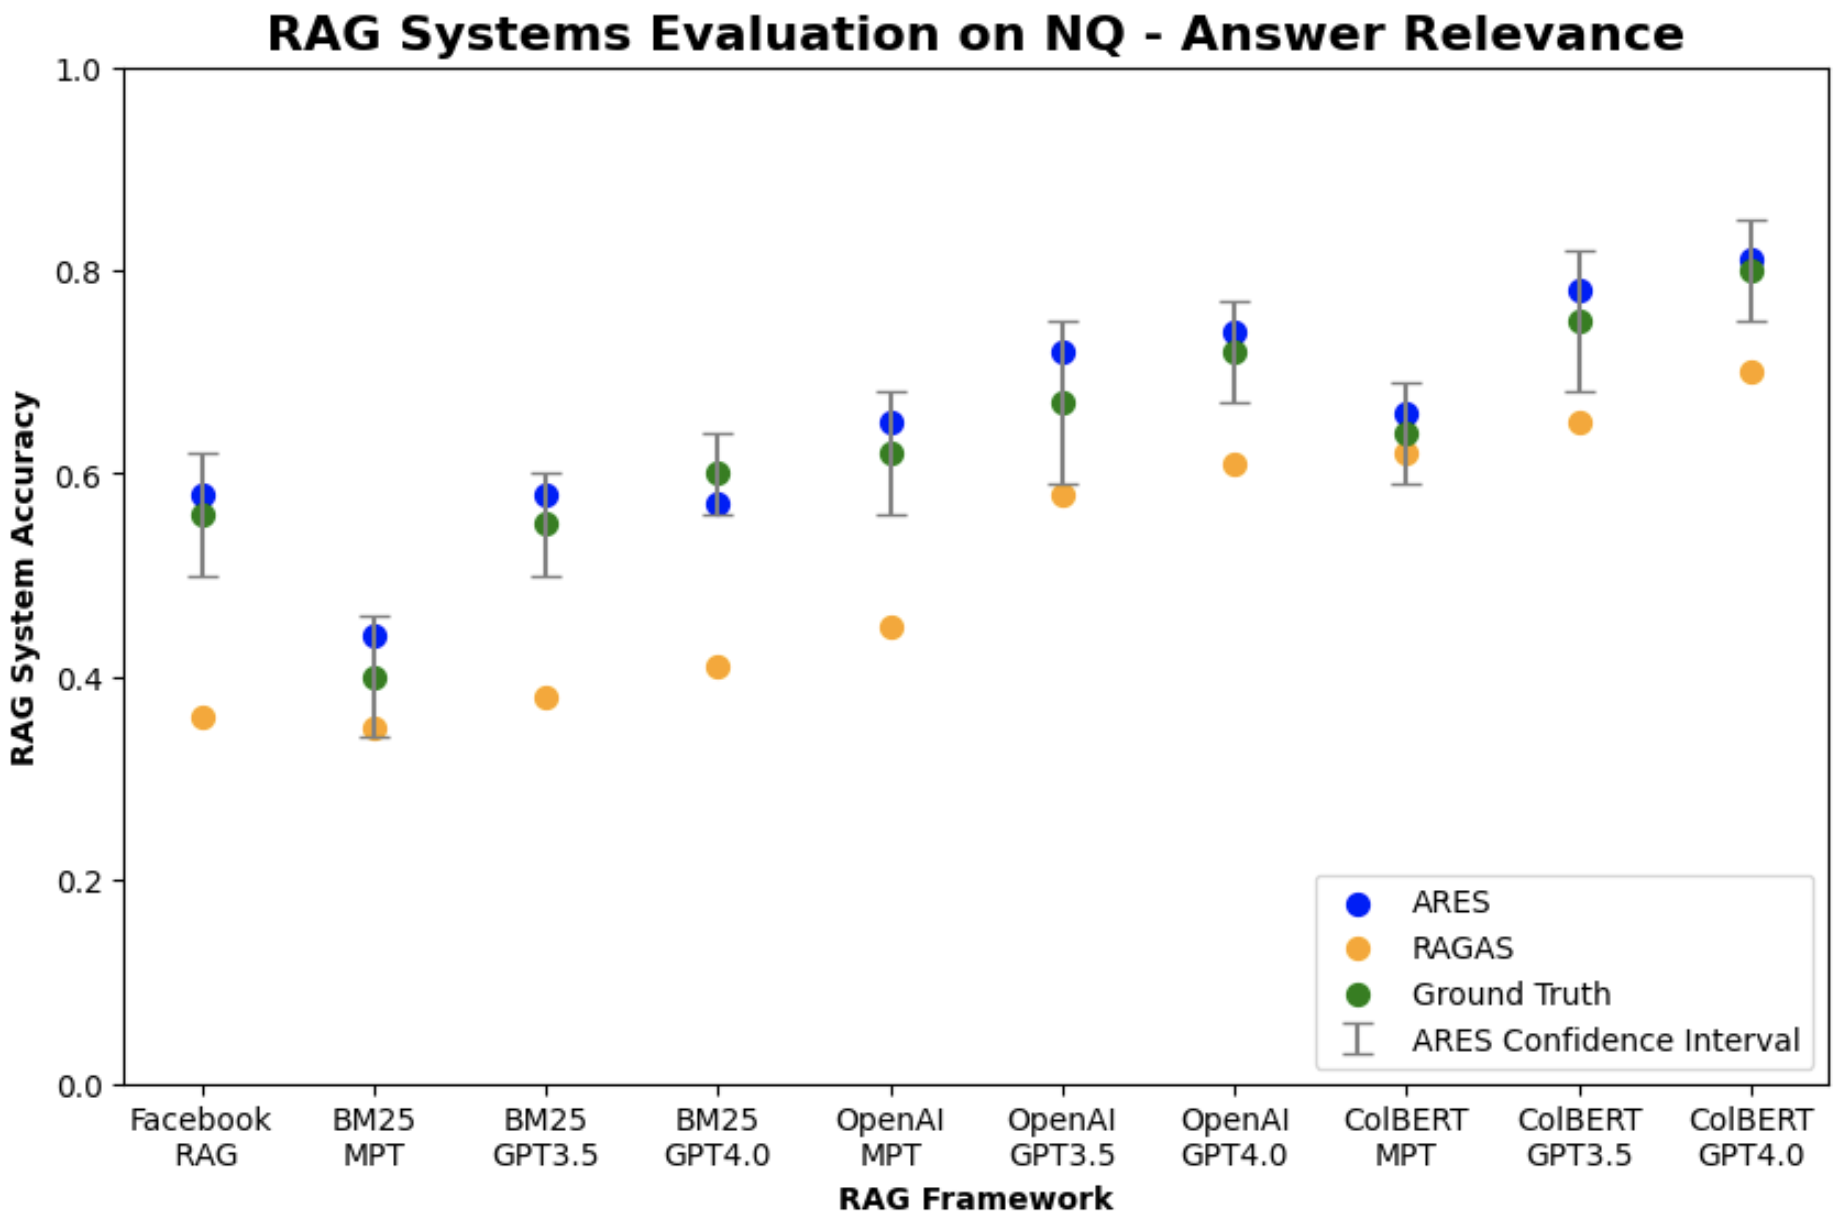
\includegraphics[width=0.8\linewidth]{Tables/NQ_AnswerRelevance.png}
   \caption{\textbf{RAG Systems Evaluation on NQ - Answer Relevance}}
   \label{fig:nq_answer_relevance_real_rag}
\end{figure*}



\begin{table*}[htp!]
\small
\centering
\setlength{\tabcolsep}{3.5pt}
\begin{tabular}{crrrrrr}
\toprule
\multicolumn{1}{l}{}                                                 & \multicolumn{6}{c}{\textbf{\begin{tabular}[c]{@{}c@{}}Kendall's Tau by Dataset\end{tabular}}}                                                                                                                                                                                                                  \\
\cmidrule(l{7pt}r{7pt}){2-7}
\textbf{}                                                            & \multicolumn{2}{c}{NQ}                                                                                                                                            & \multicolumn{2}{c}{MultiRC} & \multicolumn{2}{c}{ReCoRD}                                                                                                                                        \\
\midrule
\textbf{\begin{tabular}[c]{@{}c@{}}PPI Labeled\\ Count\end{tabular}} & \multicolumn{1}{c}{\begin{tabular}[c]{@{}c@{}}C.R.\end{tabular}} & \multicolumn{1}{c}{\begin{tabular}[c]{@{}c@{}}A.R.\end{tabular}} & \multicolumn{1}{c}{\begin{tabular}[c]{@{}c@{}}C.R.\end{tabular}} & \multicolumn{1}{c}{\begin{tabular}[c]{@{}c@{}}A.R.\end{tabular}} & \multicolumn{1}{c}{\begin{tabular}[c]{@{}c@{}}C.R.\end{tabular}} & \multicolumn{1}{c}{\begin{tabular}[c]{@{}c@{}}A.R.\end{tabular}} \\
\midrule
400                                                                  & 1.0                                                                              & 1.0                                                                            & 0.89                                                                             & 0.94  & 0.89 & 0.94                                                                          \\
300                                                                  & 0.89                                                                             & 1.0                                                                            & 0.94                                                                             & 0.89   & 0.83 & 0.89                                                                         \\
200                                                                  & 0.83                                                                             & 1.0                                                                            & 0.83                                                                             & 0.94  & 0.83 &  0.83                                                                         \\
150                                                                  & 0.72                                                                             & 1.0                                                                            & 0.83                                                                             & 0.89    & 0.72 &  0.83                                                                      \\
100                                                                  & 0.44                                                                             & 1.0                                                                            & 0.67                                                                             & 0.67  & 0.67 & 0.83                                                                          \\
50                                                                   & 0.44                                                                             & 0.94                                                                           & 0.61                                                                             & 0.44   & 0.56 & 0.67                                                                         \\
25                                                                   & 0.44                                                                             & 0.89                                                                           & 0.56                                                                             & 0.44 & 0.44 & 0.56   \\ \bottomrule                                                                        
\end{tabular}
\caption{\textbf{Analysis of PPI Labeled Count vs. ARES Efficacy by Kendall's Tau}: The Kendall's tau values represent the correlation between the correct ranking and the ARES ranking of the pseudo RAG systems. We use the same experimental set-up as described in \autoref{sec:datasets}. We find that below about 100-150 datapoints in the human preference validation set, ARES cannot meaningfully distinguish between the alternate RAG systems based on their accuracies in context relevance and answer relevance (C.R. and A.R., respectively).}
\label{tab:ppi_count}
\end{table*}



\begin{table*}[]
\small
\centering
\setlength{\tabcolsep}{2.0pt}
\begin{tabular}{lrrrrrr}
\toprule
                                                                                     & \multicolumn{6}{c}{\textbf{ARES Ranking of Pseudo RAG Systems using GPT-4 Labels}}                                                                                                                                                                                                                                                                                                                                                                                                                     \\ \cmidrule(l{7pt}r{7pt}){2-7}
                                                                                     & \multicolumn{2}{c}{NQ}                                                                                                                                           & \multicolumn{2}{c}{ReCoRD}                                                                                                                                        & \multicolumn{2}{c}{MultiRC}                                                                                                                                      \\
                                                                                     \\ \cmidrule(l{7pt}r{7pt}){2-7}
                                                                                     & \multicolumn{1}{c}{\begin{tabular}[c]{@{}c@{}}Context\\ Relevance\end{tabular}} & \multicolumn{1}{c}{\begin{tabular}[c]{@{}c@{}}Answer\\ Relevance\end{tabular}} & \multicolumn{1}{c}{\begin{tabular}[c]{@{}c@{}}Context\\ Relevance\end{tabular}} & \multicolumn{1}{c}{\begin{tabular}[c]{@{}c@{}}Answer\\ Relevance\end{tabular}} & \multicolumn{1}{c}{\begin{tabular}[c]{@{}c@{}}Context\\ Relevance\end{tabular}} & \multicolumn{1}{c}{\begin{tabular}[c]{@{}c@{}}Answer\\ Relevance\end{tabular}} 
                                                                                                                                                                                                                                                                                                                                                                                                                                                                                                                                        \\ \midrule
Kendall's Tau                                                                        & 0.78                                                                            & 1.0                                                                            & 0.78                                                                           & 0.72                                                                           & 0.89                                                                            & 0.78                                                                           \\ \midrule
\begin{tabular}[c]{@{}l@{}}Kendall's Tau of \\ Human Labeled Approach\end{tabular}                                            & 0.94                                                                            & 1.0                                                                            & 0.83                                                                            & 0.89                                                                           & 0.94                                                                            & 0.89                                                                           \\
\midrule
Average PPI Range                                                                    & 9.2\%                                                                           & 6.8\%                                                                          & 8.2\%                                                                           & 9.0\%                                                                          & 7.7\%                                                                           & 8.3\%                                                                          \\ \midrule
\begin{tabular}[c]{@{}l@{}}Accuracy on \\ RAG Evaluation Sets\end{tabular} & 79.3\%                                                                          & 96.7\%                                                                         & 88.4\%                                                                          & 78.3\%                                                                         & 85.8\%                                                                          & 82.5\%  \\ \bottomrule                                                                      
\end{tabular}
\caption{\textbf{GPT-4 Labels vs. Human Labels}: We wanted to explore the practicality of using GPT-4 generated labels instead of human annotations for our human preference validation set in ARES.
In the experiments, we generated 500 GPT-4 labels as replacements for human labeling using few-shot prompts (see Sections \ref{sec:gpt_prompting_for_context_relevance_scoring}, \ref{sec:gpt_prompting_for_answer_faithfulness_scoring}, and \ref{sec:gpt_prompting_for_answer_relevance_scoring}).
While GPT-4 generated labels decreased Kendall's tau in most settings by 0.05 to 0.30, the ability to cheaply produce GPT-4 generated labels significantly reduces the  cost of annotation, cutting it from hundreds of annotations to less than ten for few-shot prompts.
Additionally, the efficacy of PPI continues improving as we generate more GPT-4 generated labels. 
In the table, we define PPI range as the number of percentage points from the lower number to the upper number of the PPI confidence bounding. Additionally, we use the fine-tuned LLM judge (DeBERTa-v3-Large) for evaluation.}
\label{tab:gpt4_labels}
\end{table*}




\begin{table*}[]
\small
\centering
\begin{tabular}{lllllll}
\toprule
                                                                                & \multicolumn{6}{c}{\textbf{ARES Ranking of Real RAG Systems}}                                                                                                   \\
                                                                                \cmidrule(l{7pt}r{7pt}){2-7}
                                                                                & \multicolumn{2}{c}{NQ}                              & \multicolumn{2}{c}{WoW}                             & \multicolumn{2}{c}{FEVER}                           \\
                                                                                \cmidrule(l{7pt}r{7pt}){2-7}
                                                                                
\textbf{}                                                                       & \multicolumn{1}{c}{C.R.} & \multicolumn{1}{c}{A.R.} & \multicolumn{1}{c}{C.R.} & \multicolumn{1}{c}{A.R.} & \multicolumn{1}{c}{C.R.} & \multicolumn{1}{c}{A.R.} \\
\midrule
\begin{tabular}[c]{@{}l@{}}Kendall’s Tau for\\ Sampled Annotations\end{tabular} & 0.73                     & 0.78                     & 0.73                     & 0.73                     & 0.73                     & 0.82                     \\
\begin{tabular}[c]{@{}l@{}}Kendall's Tau \\ for RAGAS\end{tabular}              & 0.82                     & 0.82                     & 0.73                     & 0.82                     & 0.73                     & 0.87                     \\
\begin{tabular}[c]{@{}l@{}}Kendall's Tau\\ for GPT-3.5 Judge\end{tabular}       & 0.82                     & 0.87                     & 0.82                     & 0.82                     & 0.64                     & 0.87                     \\
\begin{tabular}[c]{@{}l@{}}Kendall's Tau\\ for ARES LLM Judge\end{tabular}      & 0.91                     & \textbf{0.96}                     & \textbf{0.91}                     & \textbf{1.0}                      & 0.73                     & 0.87                     \\
\begin{tabular}[c]{@{}l@{}}Kendall's Tau\\ for ARES\end{tabular}                & \textbf{1.0}                      & \textbf{0.96}                     & \textbf{0.91}                     & \textbf{1.0}                      & \textbf{0.82}                     & \textbf{1.0}                      \\
\midrule
RAGAS Accuracy                                                                  & 35.9\%                   & 68.2\%                   & 44.4\%                   & 80.1\%                   & 21.4\%                   & 75.9\%                   \\
GPT-3.5 Accuracy                                                                & 80.5\%                   & 91.2\%                   & 81.2\%                   & 83.5\%                   & 61.3\%                   & 54.5\%                   \\
ARES Accuracy                                                                   & 85.6\%                   & 93.3\%                   & 84.5\%                   & 88.2\%                   & 70.4\%                   & 84.0\%  \\ \bottomrule                
\end{tabular}
\caption{\textbf{ARES Ranking on Real-World RAG Systems}: 
For scoring context relevance and answer relevance (C.R. and A.R. in the table, respectively), we compare ARES with our fine-tuned LLM judges against sampled annotations benchmark, RAGAS, and a few-shot GPT-3.5 judge.
For our sampled annotations, we gather 150 annotated datapoints from each mock RAG system and use those labels to score the system.
RAGAS also uses GPT-3.5 as its judge but it uses few-shot prompts that are not targeted for each evaluation domain.
Overall, we found that ARES ranked RAG systems more accurately than RAGAS and GPT-3.5 across all the explored datasets.
Additionally, we include the Kendall's taus for the ARES LLM Judge without PPI and found that PPI further boosted the ranking accuracy of the judge across the board.
We selected GPT-3.5 instead of GPT-4 due to the lower financial costs required to run. %
For PPI in both ARES and the GPT-3.5 judge, we used 300 human annotations for our human preference validation set.
The prompts used for the GPT-3.5 judges are included in Sections \ref{sec:gpt_prompting_for_context_relevance_scoring}, \ref{sec:gpt_prompting_for_answer_faithfulness_scoring}, and \ref{sec:gpt_prompting_for_answer_relevance_scoring}.}
\label{tab:ares_real_systems}
\end{table*}


\begin{table*}[]
\small
\centering
\setlength{\tabcolsep}{1.4pt}
\begin{tabular}{lrrrrrrrrrrrr}
\toprule
                                                                                     & \multicolumn{12}{c}{\textbf{ARES Cross-Domain Ranking of Pseudo RAG Systems}}                                                                                                                                                                                                                                                                                                                                                                                                                                                                                                                                                                                                                                                                                                                                                                                                                                                                                                                 \\
                                                                                     \cmidrule(l{7pt}r{7pt}){2-13}
                                                                                     & \multicolumn{2}{c}{\begin{tabular}[c]{@{}c@{}}NQ to \\ FEVER\end{tabular}}                                                                                    & \multicolumn{2}{c}{\begin{tabular}[c]{@{}c@{}}FEVER to \\ NQ\end{tabular}}                                                                                    & \multicolumn{2}{c}{\begin{tabular}[c]{@{}c@{}}NQ to \\ MultiRC\end{tabular}}                                                                                  & \multicolumn{2}{c}{\begin{tabular}[c]{@{}c@{}}MultiRC to \\ NQ\end{tabular}}                                                                                  & \multicolumn{2}{c}{\begin{tabular}[c]{@{}c@{}}NQ to \\ ReCoRD\end{tabular}}                                                                                   & \multicolumn{2}{c}{\begin{tabular}[c]{@{}c@{}}ReCoRD to \\ NQ\end{tabular}}                                                                                   \\ \cmidrule(l{7pt}r{7pt}){2-13}
                                                                                     & \multicolumn{1}{c}{C.R.}                                                      & \multicolumn{1}{c}{A.R.}                                                      & \multicolumn{1}{c}{C.R.}                                                      & \multicolumn{1}{c}{A.R.}                                                      & \multicolumn{1}{c}{C.R.}                                                      & \multicolumn{1}{c}{A.R.}                                                      & \multicolumn{1}{c}{C.R.}                                                      & \multicolumn{1}{c}{A.R.}                                                      & \multicolumn{1}{c}{C.R.}                                                      & \multicolumn{1}{c}{A.R.}                                                      & \multicolumn{1}{c}{C.R.}                                                      & \multicolumn{1}{c}{A.R.}                                                                                                                                                                                                                                                                                                                                                                                                                                                                                                                                                                                                                                                                                                                                                                                                                                                                                                                                                                                             \\
\midrule
Kendall's Tau                                                                        & 0.89                                                                          & 0.89                                                                          & 1.0                                                                           & 0.83                                                                          & 0.94                                                                          & 0.89                                                                          & 1.0                                                                           & 0.89                                                                          & 0.78                                                                          & 0.89                                                                          & 0.89                                                                          & 0.94                                                                          
\\ \midrule
\begin{tabular}[c]{@{}l@{}}Kendall's Tau of\\ In-Domain LLM Judge\end{tabular}       & 0.89                                                                          & 0.78                                                                          & 0.94                                                                          & 1.0                                                                           & 0.94                                                                          & 0.89                                                                          & 0.94                                                                          & 1.0                                                                           & 0.83                                                                          & 0.89                                                                          & 0.94                                                                          & 1.0                                                                           \\
\midrule
Average PPI Range                                                                    & 8.7\%                                                                         & 7.2\%                                                                         & 6.5\%                                                                         & 11.5\%                                                                        & 10.2\%                                                                        & 11.3\%                                                                        & 11.9\%                                                                        & 11.5\%                                                                        & 10.5\%                                                                        & 10.1\%                                                                        & 9.7\%                                                                         & 6.2\%                                                                         \\
\midrule
\begin{tabular}[c]{@{}l@{}} Accuracy on \\ RAG Evaluation Sets\end{tabular} & 92.4\%                                                                        & 28.4\%                                                                        & 85.7\%                                                                        & 22.6\%                                                                        & 81.5\%                                                                        & 92.1\%                                                                        & 87.6\%                                                                        & 80.2\%                                                                        & 29.1\%                                                                        & 81.2\%                                                                        & 80.1\%                                                                        & 92.1\%                                                                       \\ \bottomrule
\end{tabular}
\caption{\textbf{Cross-Domain Usage of Fine-tuned LLM Judges}: We tested the cross-domain application of the fine-tuned LLM judge in the ARES framework. We found that for both context relevance and answer relevance (C.R. and A.R. in the table, respectively), fine-tuned LLM judges showed strong generalizability across domains when changing query type (e.g. NQ and FEVER), document type (e.g. NQ and MultiRC), or both (e.g. NQ and ReCoRD). For PPI, we used 300 labeled examples for our human preference validation set but also found that additional examples further improved the performance of ARES. Furthermore, we found that even in scenarios where the fine-tuned LLM judge's accuracy significantly dropped out-of-domain (e.g. answer relevance for NQ to FEVER), PPI mitigated the decrease in judge performance. In the table, we define PPI range as the number of percentage points from the lower bound to the upper bound of the PPI confidence interval.}
\label{tab:cross_domain}
\end{table*}





\begin{table*}[]
\tiny
\centering
\begin{tabular}{|l|l|l|l|l|}
\hline
\multicolumn{1}{|c|}{\textbf{Query}}                                                                                               & \multicolumn{1}{c|}{\textbf{Passage}}                                                                                                                                                                                                                                                                                                                                                                                                                                                                                                                                                                                                                                                                                                                                                                                                                                                                                                                                                                                    & \multicolumn{1}{c|}{\textbf{Answer}}                                                                        & \multicolumn{1}{c|}{\textbf{\begin{tabular}[c]{@{}c@{}}Context\\ Relevance\end{tabular}}} & \multicolumn{1}{c|}{\textbf{\begin{tabular}[c]{@{}c@{}}Answer\\ Relevance\end{tabular}}} \\ \hline
\begin{tabular}[c]{@{}l@{}}How can a ball that is not \\ moving possess energy \\ of position?\end{tabular}                        & \begin{tabular}[c]{@{}l@{}}Mechanical energy is a combination of the energy of motion or position. \\ This type of energy describes objects that are moving or could move. \\ A moving ball can have energy from motion. An arrow can also have \\ the energy of motion. Both are types of mechanical energy.\end{tabular}                                                                                                                                                                                                                                                                                                                                                                                                                                                                                                                                                                                                                                                                                               & \begin{tabular}[c]{@{}l@{}}The ball holds \\ mechanical energy\end{tabular}                                 & 1                                                                                         & 1                                                                                        \\ \hline
\begin{tabular}[c]{@{}l@{}}Who has a Jimmy\\  Stewart-like quality \\ of quiet trust?\end{tabular}                                 & \begin{tabular}[c]{@{}l@{}}One look at Fred Rooney, and you just know he's the good guy. \\ A trace of childish innocence in his face gives the lanky \\ Bethlehem lawyer a Jimmy Stewart-like quality of quiet trust. \\ In black jeans and button-down shirt, he's a kind of folk hero \\ in the south Bethlehem melting pot where he's crafted a law \\ practice catering to working-class families - mostly Latino - \\ in the shadow of the hulkish remnants of Bethlehem Steel.\end{tabular}                                                                                                                                                                                                                                                                                                                                                                                                                                                                                                                       & Fred Rooney                                                                                                 & 1                                                                                         & 1                                                                                        \\ \hline
\begin{tabular}[c]{@{}l@{}}Before he murder the \\ doctor and Ralph Smith, \\ where did the stepfather \\ reside?\end{tabular}     & \begin{tabular}[c]{@{}l@{}}Surviving being shot and stabbed at the end of the previous film , \\ the stepfather has been institutionalized in Puget Sound, Washington since , \\ spending his time building model houses in the workshop.\\ Assigned a new doctor named Joseph Danvers the stepfather \\ begins confiding in him to gain his trust , ultimately murdering \\ the doctor during a session by stabbing him in the neck with a \\ blade smuggled out of the workshop . After killing Danvers the stepfather \\ beats a suspicious guard named Ralph Smith to death with his own nightstick \\ with only two strikes and takes his uniform , successfully \\ sneaking out of the sanitarium . Checking into a hotel after robbing and \\ murdering a traveling salesman the stepfather alters his appearance , \\ takes the name Doctor Gene F. Clifford from the newspaper obituaries \\ and travels to Palm Meadows , Los Angeles after seeing an ad for it on \\ an episode of Dream House .\end{tabular} & Los Angeles                                                                                                 & 1                                                                                         & 0                                                                                        \\ \hline
\begin{tabular}[c]{@{}l@{}}What was the name of the \\ 2006 film about Pushkin's death, \\ and who portrayed Pushkin?\end{tabular} & \begin{tabular}[c]{@{}l@{}}After arriving in New York City, Einstein was taken to various places and \\ events, including Chinatown, a lunch with the editors of the New York \\ Times, and a performance of Carmen at the Metropolitan Opera, \\ where he was cheered by the audience on his arrival. \\ During the days following, he was given the keys to the city by Mayor \\ Jimmy Walker and met the president of Columbia University, who \\ described Einstein as "The ruling monarch of the mind." Harry \\ Emerson Fosdick, pastor at New York's Riverside Church, gave \\ Einstein a tour of the church and showed him a full-size statue that \\ the church made of Einstein, standing at the entrance.\end{tabular}                                                                                                                                                                                                                                                                                        & \begin{tabular}[c]{@{}l@{}}Vasily Szaitsev portrayed \\ Pushkin in the film \\ Pushkin Returns\end{tabular} & 0                                                                                         & 0                                                                                        \\ \hline
\end{tabular}
\caption{Positive and Negatives Evaluation Examples}
\label{tab:positive_negative_examples}
\end{table*}
